\documentclass[UTF8]{beamer}
\usepackage[utf8]{inputenc}
\usepackage[normalem]{ulem}
\usepackage{xeCJK}
\usepackage{
    amsmath, amssymb, listings, hyperref,
    subcaption, float, booktabs, csquotes,
    enumitem, tikz, pgf, pgfplots, cancel,
    ulem, fancyhdr, framed, amsthm, mathtools,
    ifsym
}

\setCJKmainfont[BoldFont=Songti SC Bold]{Songti SC Regular}
\setCJKsansfont{Heiti SC}
\setCJKmonofont{Courier}

\newcommand{\figc}[2]{
\begin{figure}[H]\begin{center}
    #1
    \caption{#2}
\end{center}\end{figure}
}

\usetikzlibrary{arrows, automata}
\AtBeginEnvironment{align}{\setcounter{equation}{0}}

\theoremstyle{plain}
%\newtheorem{theorem}{Theorem}
%\newtheorem*{theorem*}{Theorem}
%\newtheorem{lemma}{Lemma}


\theoremstyle{definition}
\newtheorem*{claim}{Claim}
\newtheorem{defn}{Definition}

\theoremstyle{remark}
\newtheorem{remark}{Remark}


\newcommand{\ffig}[2]{
\begin{figure}[H]\begin{center}
    #1
    \caption{#2}
\end{center}\end{figure}
}
\newcommand\m[1]{\begin{bmatrix}#1\end{bmatrix}}
\newcommand\mc[1]{\mathcal{#1}}
\newcommand\mb[1]{\mathbf{#1}}

\definecolor{dkgreen}{rgb}{0,0.6,0}
\definecolor{gray}{rgb}{0.5,0.5,0.5}
\definecolor{mauve}{rgb}{0.58,0,0.82}

\lstset{
  language=matlab,
  aboveskip=3mm,
  belowskip=3mm,
  showstringspaces=false,
  columns=flexible,
  basicstyle={\small\ttfamily},
  numbers=left,
  numberstyle=\tiny\color{gray},
  keywordstyle=\color{blue},
  commentstyle=\color{dkgreen},
  stringstyle=\color{mauve},
  breaklines=true,
  breakatwhitespace=true
  tabsize=2
}

\makeatletter
\renewcommand*\env@matrix[1][*\c@MaxMatrixCols c]{%
   \hskip -\arraycolsep
   \let\@ifnextchar\new@ifnextchar
   \array{#1}}
\makeatother

\newcommand*{\bc}{\Leftrightarrow}
\newcommand*{\then}{\Rightarrow}
\newcommand*{\st}{~\middle|~}

\newcommand*{\vrbar}{\rule[-1ex]{0.5pt}{2.5ex}}
\newcommand*{\hrbar}{\rule[.5ex]{2.5ex}{0.5pt}}

\newcommand{\zerodel}{.\kern-\nulldelimiterspace}

\newcommand{\R}{\mathbb{R}}
\renewcommand{\H}{\mathbb{H}}
\newcommand{\C}{\mathbb{C}}
\newcommand{\Z}{\mathbb{Z}}
\newcommand{\Q}{\mathbb{Q}}
\newcommand{\N}{\mathbb{N}}
\newcommand{\qedb}{$\blacksquare$}
\newcommand{\blank}{\textvisiblespace}
\newcommand{\Mod}{~\mathrm{mod}~}

\DeclareMathOperator{\Cl}{Cl}
\DeclareMathOperator{\POLY}{P}
\DeclareMathOperator{\NPOLY}{NP}
\DeclareMathOperator{\NPOLYC}{NP--Complete}
\DeclareMathOperator{\CONPOLY}{co--NP}
\DeclareMathOperator*{\argmax}{arg\,max}
\DeclareMathOperator*{\argmin}{arg\,min}
\DeclareMathOperator*{\rank}{rank}
\DeclareMathOperator*{\spn}{span}
\DeclareMathOperator*{\Arg}{Arg}
\DeclareMathOperator*{\im}{Im}
\DeclareMathOperator*{\lcm}{lcm}
\DeclareMathOperator*{\sgn}{sgn}

\DeclarePairedDelimiterX{\inp}[2]{\langle}{\rangle}{#1, #2}


\usetheme{Madrid}

\AtBeginSection[]{
  \begin{frame}
  \vfill
  \centering
  \begin{beamercolorbox}[sep=8pt,center,shadow=true,rounded=true]{title}
    \usebeamerfont{title}\insertsectionhead\par%
  \end{beamercolorbox}
  \vfill
  \end{frame}
}

\pgfplotsset{every axis/.append style={
                    axis x line=middle,    % put the x axis in the middle
                    axis y line=middle,    % put the y axis in the middle
                    axis line style={->}, % arrows on the axis
                    xlabel={$x$},          % default put x on x-axis
                    ylabel={$y$},          % default put y on y-axis
                    }}

\usefonttheme{serif}
\title{Kolmogorov-Arnold Networks}
\author{jhl}
\institute[]{@c/sim-aaa $\cdot$ @ucsd}
\date{10 June 2024}

\begin{document}

{
\setbeamertemplate{footline}{} 
\begin{frame}{}
    {\center Sim-Eval Literature Review}
    \titlepage
\end{frame}
}

\addtocounter{framenumber}{-1}

\begin{frame}{Welcome to the inaugural Sim-Eval literature review!} 
    I'm trying to keep this informal -- teaching is the best way of learning,
    and we all benefit from sharing knowledge. (I also only had a weekend to prepare.) 
    \textbf{Some bookkeeping notes:}
    \begin{itemize}
        \item Expect a bit more of the underlying intuition here, instead of the mechanical
            $\varepsilon-\delta|_{n \to \infty}$ aspects of the proofs.
        \item For simplicity, assume that the functions we care about are
            \textit{of multiple variables} and \textit{scalar-valued}, i.e. 
            \[
                f: \R^n \longrightarrow \R
            \]
        \item This talk is motivated by a recent paper by Liu, Wang et al. It is accessible
         at \url{https://arxiv.org/pdf/2404.19756v1}. Unless otherwise stated, 
         figures are credited to Liu et al.
    \end{itemize}
\end{frame}

\section{A gentle (re)introduction to the multi-layer perceptron}

\begin{frame}

    The multi-layer perceptron (MLP) is the fundamental building block of
    so-called deep neural networks. Deep refers to the large ``depth'' of the network, i.e. 
    the number of layers.

    \ffig{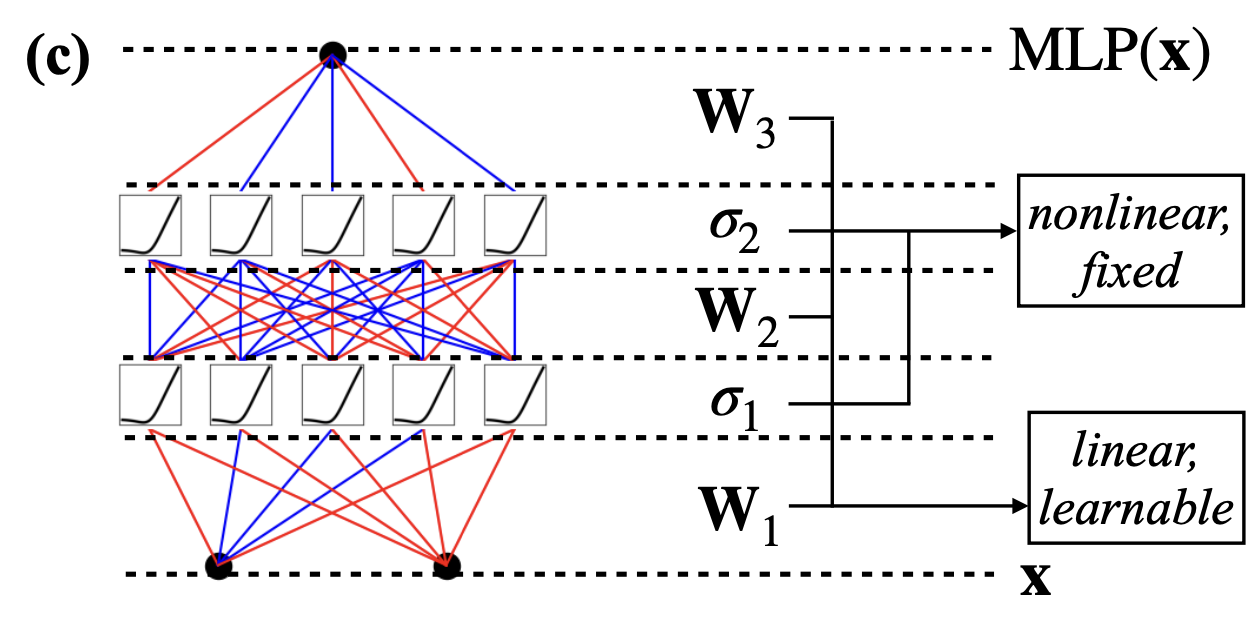
\includegraphics[width=6cm]{deepmlp}}{\textit{A deep multi-layer perceptron network.}}
\end{frame}

\begin{frame}
    Canonically, a ``shallow'' multi-layer perceptron is \textit{two layers}. (This will be important
    for the literature!)
    A multi-layer perceptron in the shallow case is represented as
    \begin{align*}
        \hat{f} &: ~ \R^n \longrightarrow \R \\
        \hat{f}(x) &=  \sum_i^{N(\varepsilon)} a_i \sigma \left[\mathbf{W}_i \mathbf{x} + b_i \right]
    \end{align*}
    Note the width $N(\varepsilon)$ is a function of the precision $\varepsilon$.
\end{frame}

\begin{frame}
    \begin{align*}
        \hat{f}(x) &=  \sum_i^{N(\varepsilon)} a_i \sigma \left[\mathbf{W}_i \mathbf{x} + b_i \right]
    \end{align*}
    where:
    \[
        \begin{array}{c|l}
            b_i & \text{is the bias \textit{(affine!)}} \\
            \mathbf{x} & \text{is the $i$ th input vector} \\
            \mathbf{W}_i & \text{is the $i$ th weight matrix \textit{(learned!)}} \\
            \sigma & \text{is the activation function \textit{(e.g. ReLU, sigmoid, $\tanh$...)}} \\
            a_i & \text{are elements of the outermost weight matrix} \\
            N(\varepsilon) & \text{is the number of neurons}
        \end{array}
    \]
    In the shallow case, $a_i$ can be denoted by a row vector.
\end{frame}
\begin{frame}
    \begin{align*}
        \hat{f}(x) &=  \sum_i^{N(\varepsilon)} a_i \sigma \left[\mathbf{W}_i \mathbf{x} + b_i \right]
    \end{align*}
    \ffig{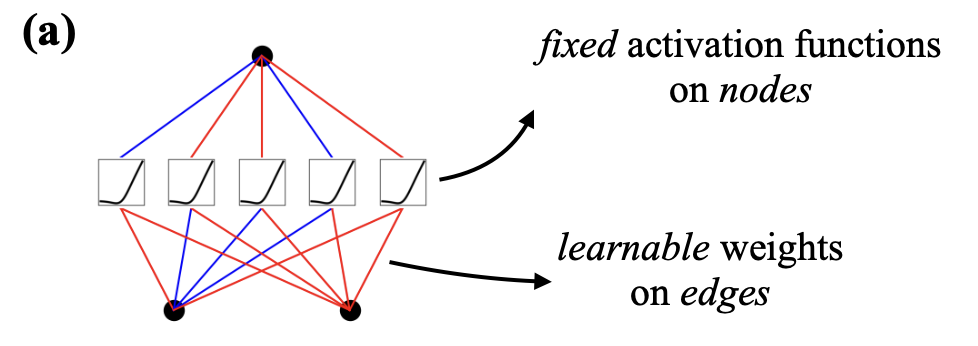
\includegraphics[width=6cm]{shallowmlp}}{\textit{A shallow 2-layer multi-layer perceptron.} $d=2$, $n=5$.}
\end{frame}
\begin{frame}
    More generally, for deep ($d > 2$) networks, a multi-layer perceptron is
    really just a composition of (affine!) linear transformations separated by non-linear
    activations.
    \[
        MLP(x) = \left[
            W_d \circ \sigma_d \circ
            W_{d-1} \circ \sigma_{d-1} \circ
                \ldots
            W_{1} \circ \sigma_{1} 
        \right] (x)
    \]
    \ffig{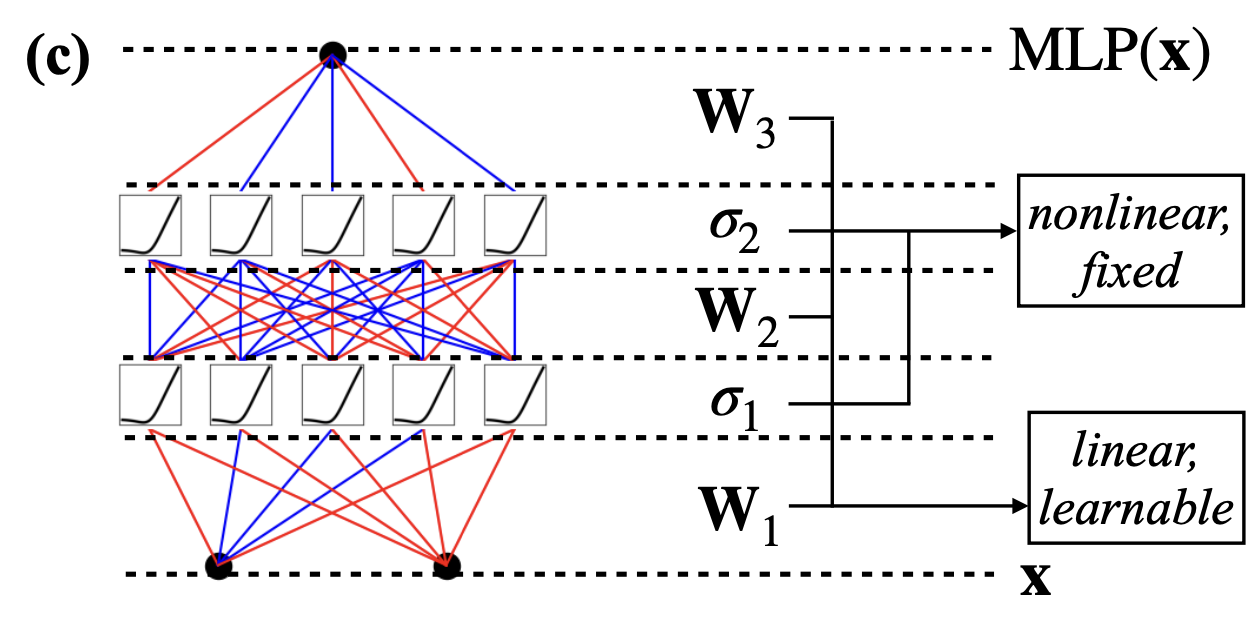
\includegraphics[width=6cm]{deepmlp}}{\textit{A deep multi-layer perceptron network.}}
\end{frame}

\begin{frame}
    \[
        \hat{f}(x) =  \sum_i^{N(\varepsilon)} a_i \sigma \left[\mathbf{W}_i \mathbf{x} + b_i \right]
    \]
    \textbf{\textit{Question:}} What can a multi-layer perceptron represent? \\
    \ffig{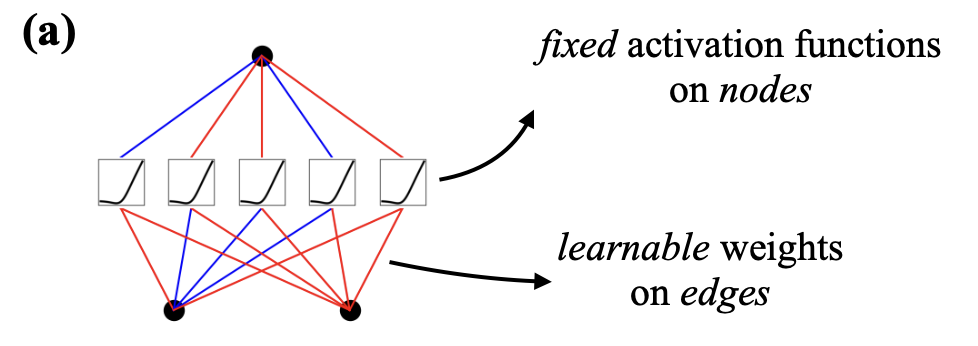
\includegraphics[width=6cm]{shallowmlp}}{\textit{A shallow 2-layer multi-layer perceptron.} $d=2$, $n=5$.}
\end{frame}

\section{Universal Approximation}

\begin{frame}
    \textbf{\textit{Question:}} What can a multi-layer perceptron represent? \\
    \textbf{\textit{Answer}} Anything!$^*$ \\
    \vspace{1cm}
    Let $D \subset \R^n$ be compact\footnote{\tiny
        Compact denotes some notion of ``closed and bounded'' -- the $n$-dimensional
        equivalent of a closed interval $[a, b] \subset \R$.
    }.
    $f: D \longrightarrow \R$ be an \textit{arbitrary nonlinear function}, and let $\hat{f}: D \longrightarrow
    \R$ denote a shallow (\textit{n.b.} 2-layer) multi-layer perceptron, denoted by
    \[
        \hat{f}(x) =  \sum_i^{N(\varepsilon)} a_i \sigma \left[\mathbf{W}_i \mathbf{x} + b_i \right]
    \]
    where $N(\varepsilon)$ is the \textit{number of neurons}. In the shallow case this is $=$ 
    the width.
\end{frame}
\begin{frame}
    Let $D \subset \R^n$ be compact.
    $f: D \longrightarrow \R$ be an \textit{arbitrary nonlinear function}, and let $\hat{f}: D \longrightarrow
    \R$ denote a shallow (\textit{n.b.} 2-layer) multi-layer perceptron, denoted by
    \[
        \hat{f}(x) =  \sum_i^{N(\varepsilon)} a_i \sigma \left[\mathbf{W}_i \mathbf{x} + b_i \right]
    \]
    \begin{theorem}
        \textbf{Universal approximation (2-layer network).} For arbitrary $\varepsilon \in \R > 0$, there
        exists $N(\varepsilon)$ such that 
        \[
        |f(x) - \hat{f(x)}| \leq \varepsilon
        \]
    \end{theorem}
\end{frame}

\begin{frame}
    \[
        \hat{f}(x) =  \sum_i^{N(\varepsilon)} a_i \sigma \left[\mathbf{W}_i \mathbf{x} + b_i \right]
    \]
    \begin{theorem}
        \textbf{Universal approximation (2-layer network).} For arbitrary $\varepsilon \in \R > 0$, there
        exists $N(\varepsilon)$ such that 
        \[
        |f(x) - \hat{f(x)}| \leq \varepsilon
        \]
    \end{theorem}
    So we can model basically anything! But...
\end{frame}

\begin{frame}
    \begin{theorem}
        \textbf{Universal approximation (2-layer network).} For arbitrary $\varepsilon \in \R > 0$, there
        exists $N(\varepsilon)$ such that 
        \[
        |f(x) - \hat{f(x)}| \leq \varepsilon
        \]
    \end{theorem}
    ...the practical question is:
    \begin{center}
        \textbf{What is $N(\varepsilon)$?}
    \end{center}
    Is it $O(\log \varepsilon^{-1})$? $O(\varepsilon^{-1})$? $O(\exp \varepsilon^{-1})$?
\end{frame}
\section{Neural scaling}
\begin{frame}
    \textbf{What is $N(\varepsilon)$?}
    \\
    \textbf{We don't know, in general!} The universal approximation theorem guarantees no bounds on $N$. 
    For deep networks,
    we do know that it's possibly poorly behaved ($N \propto \exp(d)$, the layer depth of the network).
\end{frame}

\begin{frame}
    \textbf{Why does this make sense?} Because we are fitting a ``mostly linear'' model to an ``arbitrary
    non-linear'' function. We need ``a lot of linear pieces'' to get good at modeling funky nonlinear functions.

    \ffig{
        \begin{tikzpicture}[yscale=0.3]
            \draw[thick,->] (-4.8, 0) -- (4.8, 0);
            \draw[thick,->] (0, -1.8) -- (0, 13.8);
            \draw[step=2cm,very thin,color=gray] (-4.6, -1.1) grid (4.6, 12.1);
            \draw[--] (-3, 0.3) -- (-3, -0.3) node [below=1mm] {-3};
            \draw[--] (3, 0.3) -- (3, -0.3) node [below=1mm] {3};
            \draw (3.7, 14) node [below=2mm,right=1mm,fill=white,text=red] (quad) {$f = x^2$};
            \draw (3.5, 11.5) node [below=4mm,right=1mm,fill=white,text=blue] (quad) {$\hat{f} \approx x^2$};
            \begin{scope}
                \draw[red,thick,->] plot [domain=-3.7:3.7] ({\x}, {\x * \x});
            \end{scope}
            \draw[blue, <-] (3.5, 11.5) -- (3, 9) -- (2, 4) -- (1, 1) -- (0, 0) -- (-1, 1) -- (-2, 4) -- (-3, 9) -- (-3.5, 11.5);
        \end{tikzpicture}
    }{\textit{It takes a lot of line segments to approximate this quadratic on $[-3, 3]$, and as soon as we leave $[-3, 3]$,
    the error in our approximation blows up!}}

    Enter the notion of \textit{neural scaling laws}.
\end{frame}

\begin{frame}
    Neural scaling laws formalize the notion of ``mostly linear things approximate nonlinearities inefficiently'' --
    in particular, we can generally say that the \textit{training}\footnote{
        i.e. overfits
    } loss $\ell$ decreases according a power-law regime:
    \[
        \ell \propto N^{-\alpha}
    \]
    where $\alpha$ is the \textit{scaling exponent} and $N$ is the number of parameters. In essence,
    to decrease the loss linearly requires an exponential increase in the number of parameters.
\end{frame}

\begin{frame}
    In essence, to decrease the loss linearly requires an exponential increase in the number of parameters. \\

    Fundamentally, if the underlying process is nonlinear, then we are basically trying to fit a big piecewise
    linear function, and then combining them with a fixed nonlinearity (ReLU, sigmoid, tanh, \&c).
    \ffig{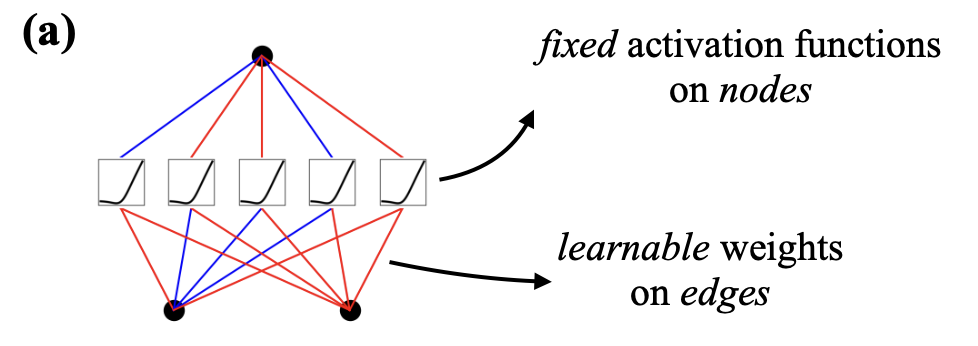
\includegraphics[width=6cm]{shallowmlp}}{\textit{The shallow perceptron again.} The nodes
        apply a fixed nonlinear activation to each input, which is a learned affine linear function
        over the incoming edges.
    }
\end{frame}

\begin{frame}
    \textbf{A practical example}: \url{go/tensorflowplayground}
    \ffig{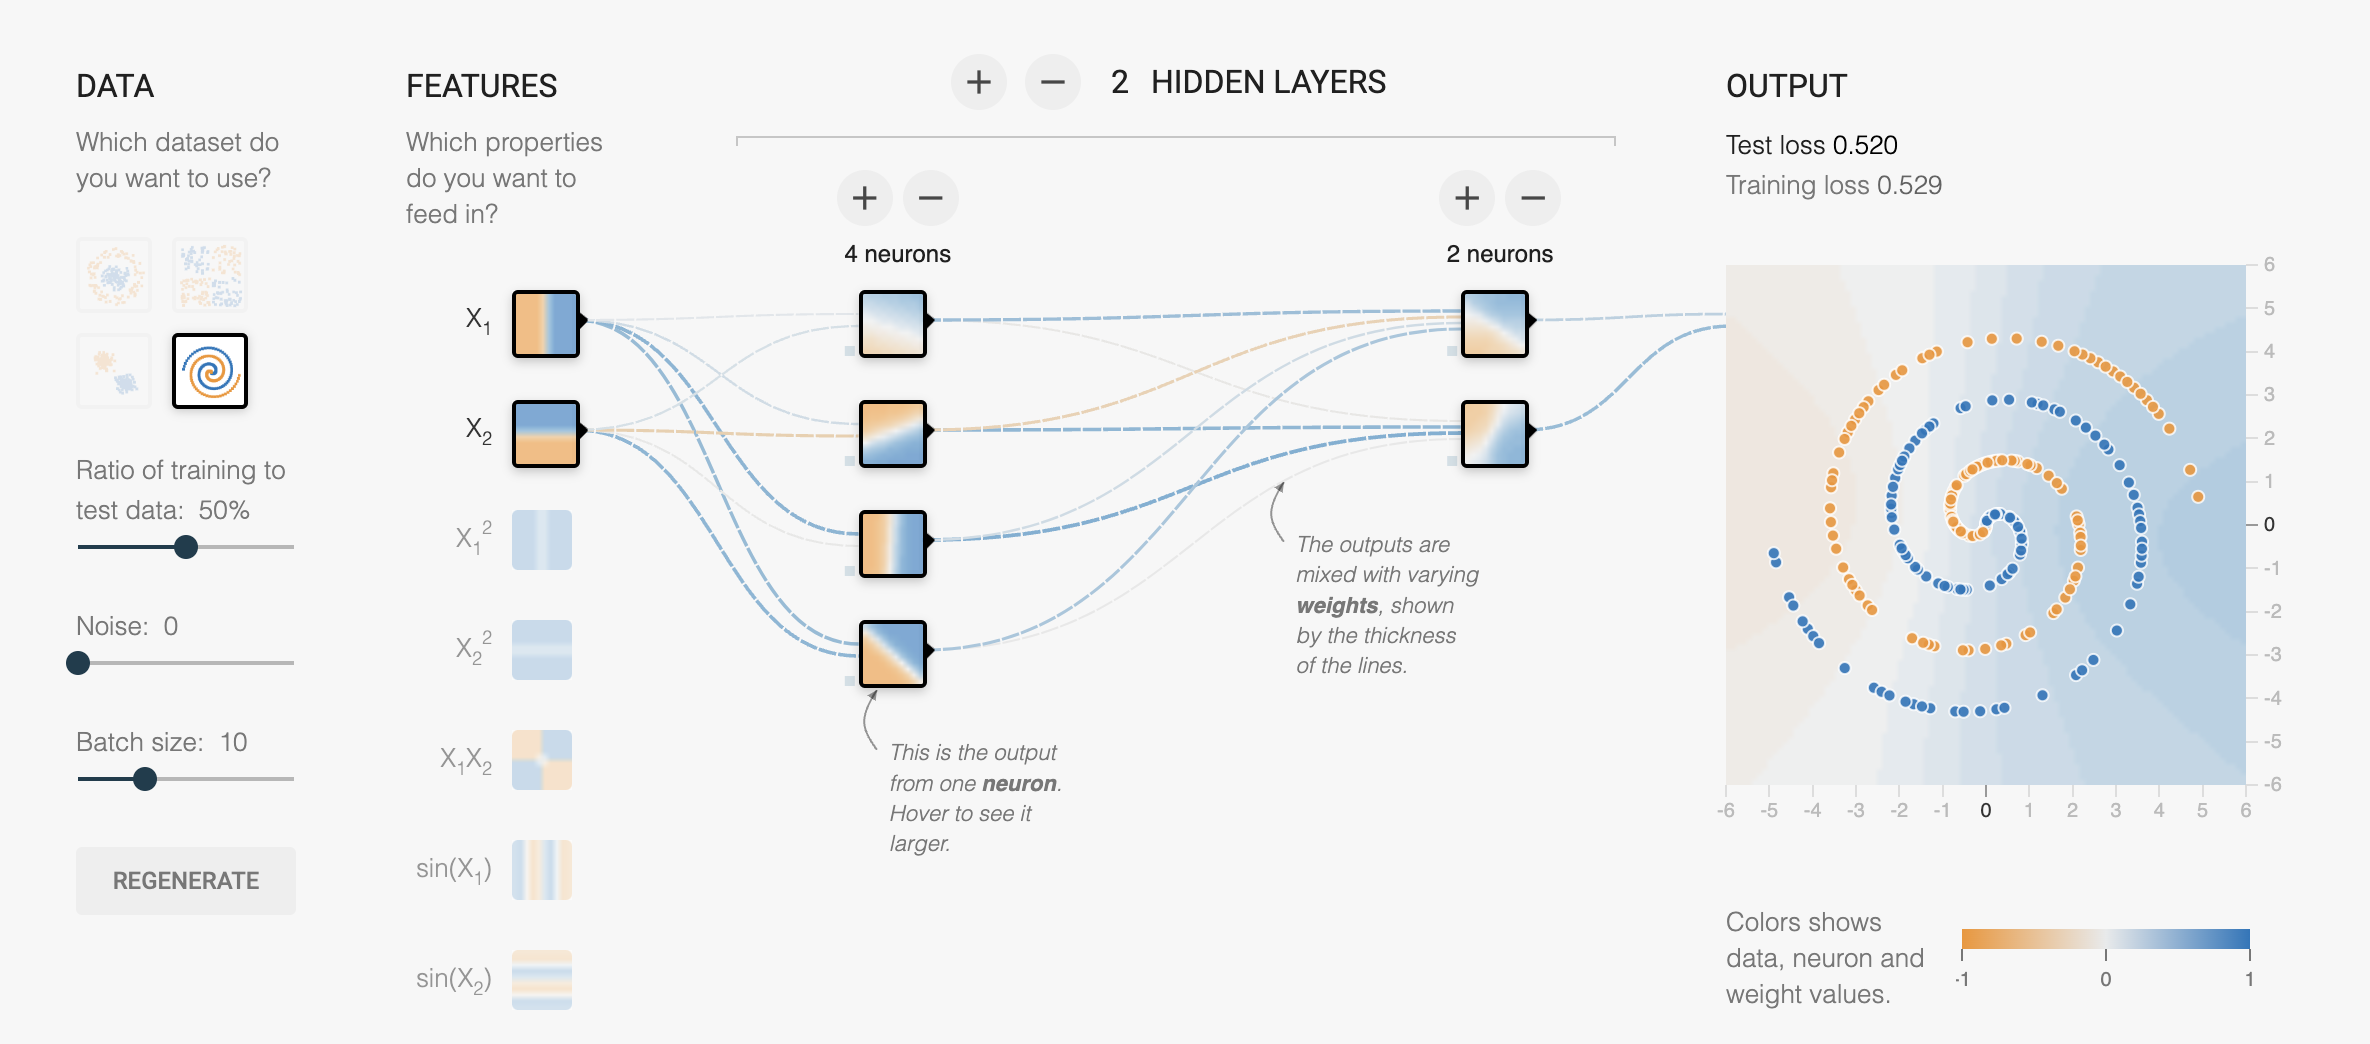
\includegraphics[width=9cm]{tfspiral}}{\textit{Separating linearly inseparable data, with linear functions?}}
\end{frame}

\begin{frame}
    \textbf{Idea:} Why not \textit{learn the nonlinearity}? \\
    \vspace{5mm}
    Using linear piecewise bits to represent a nonlinear function seems impractical. Besides, we already
    use nonlinear basis functions to fit models (e.g. polynomial degree-$n$ regression, exponential
    regression, spline fitting). \\
    \vspace{5mm}
    This is the basic idea behind the Kolmogorov-Arnold network.
\end{frame}

\section{Kolmogorov-Arnold representation}

\begin{frame}
    The fundamental architectural difference (other than learning the nonlinear
    `activation') between the multi-layer perceptron and the Kolmogorov-Arnold
    network is that nodes and edges are flipped:
    \ffig{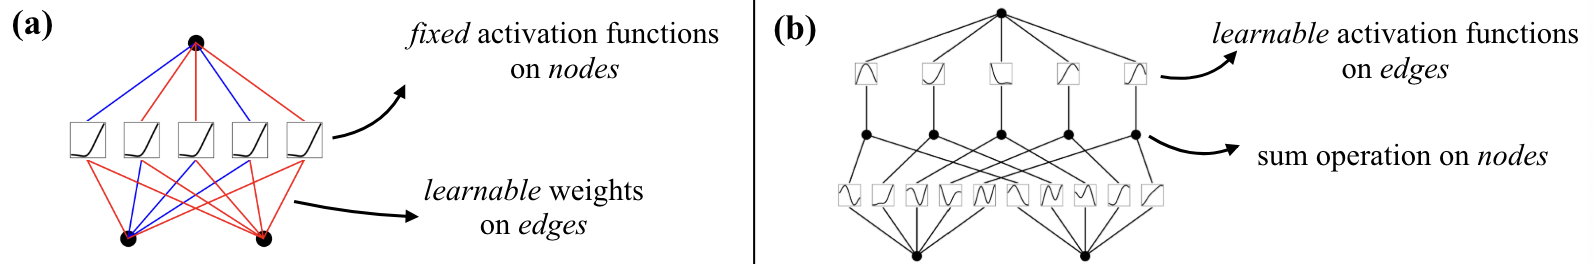
\includegraphics[width=12cm]{mlpvskan}}{\textit{MLP (right) vs. KAN (left) in the shallow case.}}
    Both of these are two-layer architectures. 
\end{frame}

\begin{frame}
    The multi-layer perceptron was underpinned by the Universal Approximation theorem. The Kolmogorov-Arnold network is
    similarly underpinned by the Kolmogorov-Arnold representation theorem (surprise). 
    Let $f$ be a continuous function defined on a closed hypercube, i.e. $f : [0,1]^n \subset \R^n \longrightarrow \R$.
    \begin{theorem}
        \textbf{Kolmogorov-Arnold representation.} $f$ admits a representation that is the sum of continuous
        functions of a single variable. In particular: there exist $\phi_{q, p} : [0, 1] \longrightarrow \R$
        and $\Phi_q: \R \longrightarrow \R$ where
        \[
            f(x) = f(x_1, x_2, \ldots x_n) = \sum_{q=0}^{2n} \Phi_q \left(
                \sum_{p=1}^n \phi_{q, p} (x_p)
                \right)
        \]
    \end{theorem}
\end{frame}

\begin{frame}
    \begin{theorem}
        \textbf{Kolmogorov-Arnold representation.} $f$ admits a representation that is the sum of continuous
        functions of a single variable. In particular: there exist $\phi_{q, p} : [0, 1] \longrightarrow \R$
        and $\Phi_q: \R \longrightarrow \R$ where
        \[
            f(x) = f(x_1, x_2, \ldots x_n) = \sum_{q=0}^{2n} \Phi_q \left(
                \sum_{p=1}^n \phi_{q, p} (x_p)
                \right)
        \]
    \end{theorem}
    Well that's abstract and unhelpful! What does it mean?
\end{frame}

\begin{frame}
    Rather surprisingly, it tells us that \textit{every multivariable function defined on a compact set
    can be written with a collection of univariate functions, composed and added together}! This is a pretty 
    remarkable result:
    \begin{align*}
        & x \in [0, 1]^n \implies \\
        & \qquad \underbrace{f(x) = f(x_1, x_2, \ldots x_n)}_{\text{multivariate}}
        = \sum_{q=0}^{2n} \underbrace{\Phi_q}_{\text{univariate}} \left(
            \sum_{p=1}^n \underbrace{\phi_{q, p}}_{\text{univariate}} (x_p)
            \right)
    \end{align*}
\end{frame}

\begin{frame}
    \begin{align*}
        & x \in [0, 1]^n \implies \\
        & \qquad \underbrace{f(x) = f(x_1, x_2, \ldots x_n)}_{\text{multivariate}}
        = \sum_{q=0}^{2n} \underbrace{\Phi_q}_{\text{univariate}} \left(
            \sum_{p=1}^n \underbrace{\phi_{q, p}}_{\text{univariate}} (x_p)
            \right)
    \end{align*}
    There is a catch: we have no guarantees on how nicely-behaved these univariate functions are.
    It could well be the case that our $\phi, \Phi$ are nondifferentiable or even fractal.
\end{frame}

\begin{frame}
    Fortunately, in practice, (it turns out) if you're modeling a real-life process, the odds are good that they will be 
    (reasonably) well-behaved. Training \textit{B-splines} turns out to be effective.\\
    \begin{defn}
        A B-spline of order $n$ is a \emph{piecewise polynomial} function of degree $n - 1$; the points
        where they meet are called \emph{knots}. It has derivatives continuous up to the degree\footnote{
            if all knots are distinct.
        } $n - 1$. B-splines can smoothly approximate any function on a compact domain to within arbitrary precision
        by interpolating between knots.
    \end{defn}
\end{frame}
\begin{frame}
    In addition, the KA theorem only discusses the shallow (2-layer) case. In
    much the same way as a deep MLP network, we can stack layers of these KAN
    networks together.
    \ffig{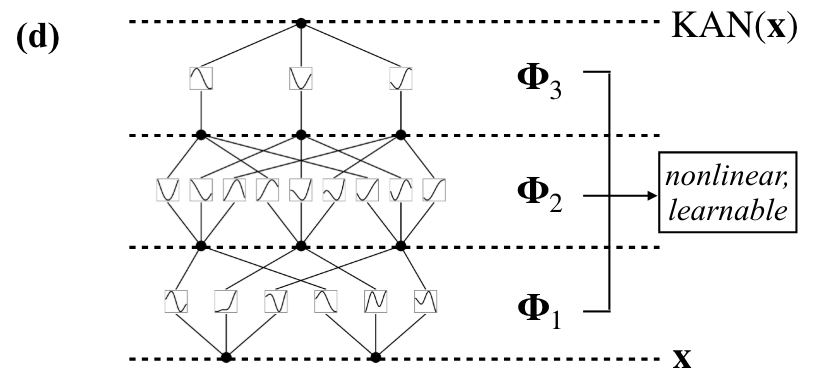
\includegraphics[width=6cm]{deepkan}}{\textit{A deep KAN.}}
\end{frame}

\begin{frame}
    \ffig{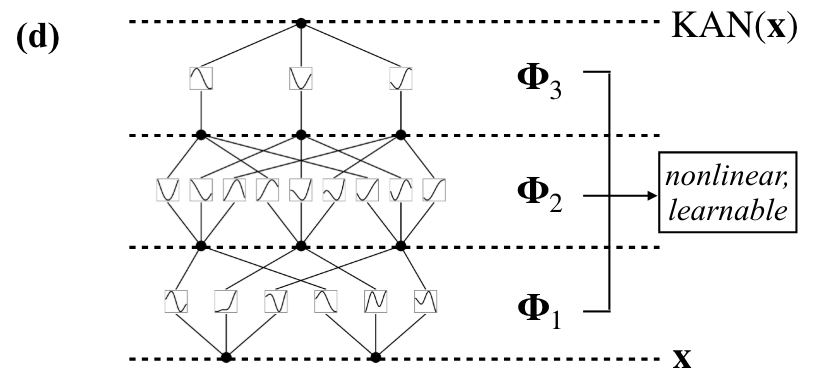
\includegraphics[width=6cm]{deepkan}}{\textit{A deep KAN.}}
    Empirically, it turns out these have high approximating power (among other benefits!).
    A deep KAN admits a very simple representation:
    \[
        \text{KAN}(x) = (\phi_d \circ \phi_{d-1} \circ \ldots \circ \phi_1)(x)
    \]
    Compare to the deep MLP formulation:
    \[
        MLP(x) = \left[
            W_d \circ \sigma_d \circ
            W_{d-1} \circ \sigma_{d-1} \circ
                \ldots
            W_{1} \circ \sigma_{1} 
        \right] (x )
    \]
\end{frame}

\begin{frame}
    From the previous discussion about neural scaling, we might expect a KAN to
    be \textit{more efficient} at representing nonlinear processes than a deep MLP.
    \\ \vspace{5mm}
    \textbf{Is this true?}
\end{frame}

\begin{frame}
    \textbf{Yes!} 
    \ffig{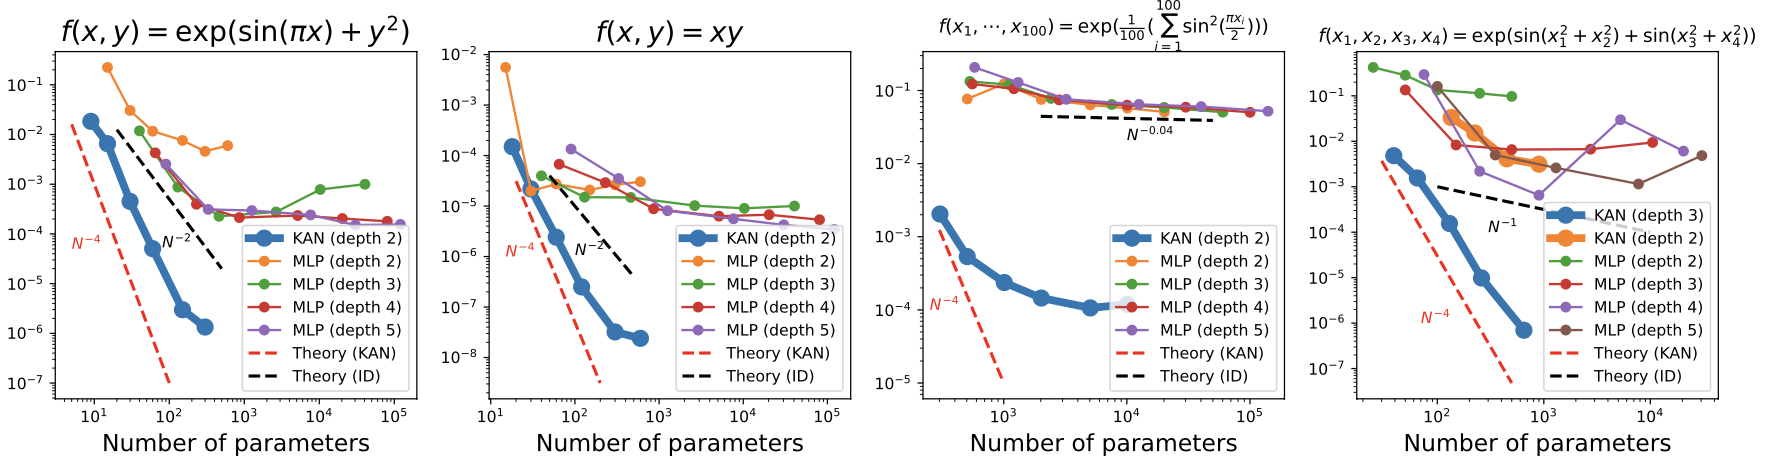
\includegraphics[width=10cm]{scaling}}{\textit{Comparison of RMSE vs. number of parameters in the KAN and MLP case.}}
    But why? (Dense theorem incoming.)
\end{frame}

\begin{frame}
    \begin{theorem}
        \textbf{Kolmogorov-Arnold, assuming continuity.} Let $x = (x_1, x_2, \ldots x_n)$, and suppose $f(x)$ admits
        a deep KA representation
        \[
        f = (\phi_{d} \circ \phi_{d - 1} \circ \ldots \phi_1)(x)
        \]
        where $\phi_k = \sum_{i = 1}^{n_k} \varphi_{z(k, i)}(x_i)$, and each $\varphi_z$ is \textbf{$k+1$ times continuously differentiable.}
        Then each $\varphi$ can be written as a sum of univariate order-K
        B-splines, and there exists $C \in \R_{\geq0}$ depending on $f$ and its
        representation that for any $0 \leq m \leq k$
        \[
            ||f - (\phi_{d}^G \circ \phi_{d-1}^G \circ \ldots \phi_1^G)||_{C^m} \leq CG^{-k-1+m}
        \]
        where $G$ is the number of knots. $|| g ||_{C^m}$ is the derivative norm equal to $\max_{|\beta| \leq m} \sup_{x \in [0, 1]^n} |D^\beta g |$.
    \end{theorem}
\end{frame}

\begin{frame}
    \[
        ||f - (\phi_{d}^G \circ \phi_{d-1}^G \circ \ldots \phi_1^G)||_{C^m} \leq CG^{-k-1+m}
    \]
    This implies that the error between a deep KAN and the underlying function is \emph{independent of dimension}. 
    KANs are \emph{free from curse of dimensionality} -- we can therefore expect (and in fact see!) better neural scaling laws. 
    \ffig{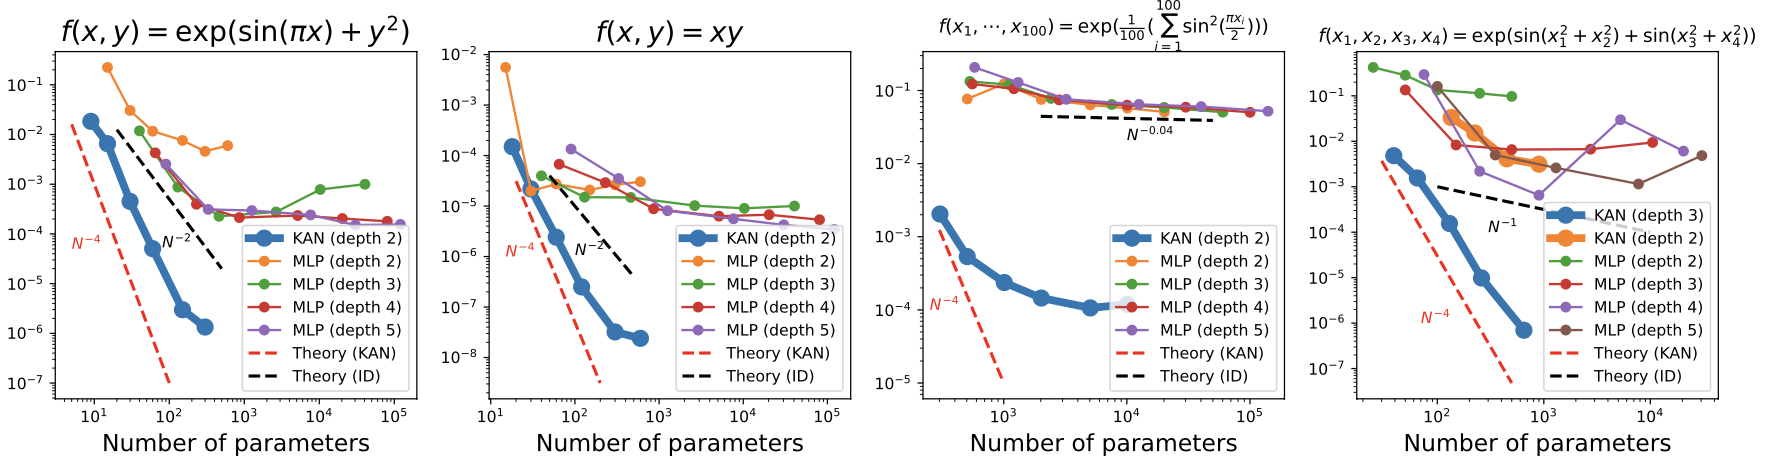
\includegraphics[width=8cm]{scaling}}{\textit{Comparison of RMSE vs. number of parameters in the KAN and MLP case.}}
\end{frame}
\begin{frame}
    \[
        ||f - (\phi_{d}^G \circ \phi_{d-1}^G \circ \ldots \phi_1^G)||_{C^m} \leq C\overbrace{G^{-(k+1)+m}}
    \]
    Further, it implies we can \textit{fine-tune the univariate representations}\footnote{
    I coin the term `eigenfeatures', but Liu et al. refer to this process as `grid extension'.}
    by increasing $G$, the number of knots, without touching the dimensionality\footnote{dimensionality, broadly, is layer or feature width} of the model!
\end{frame}
\begin{frame}
    What does a learned spline look like? It turns out they look quite intuitive:
    \ffig{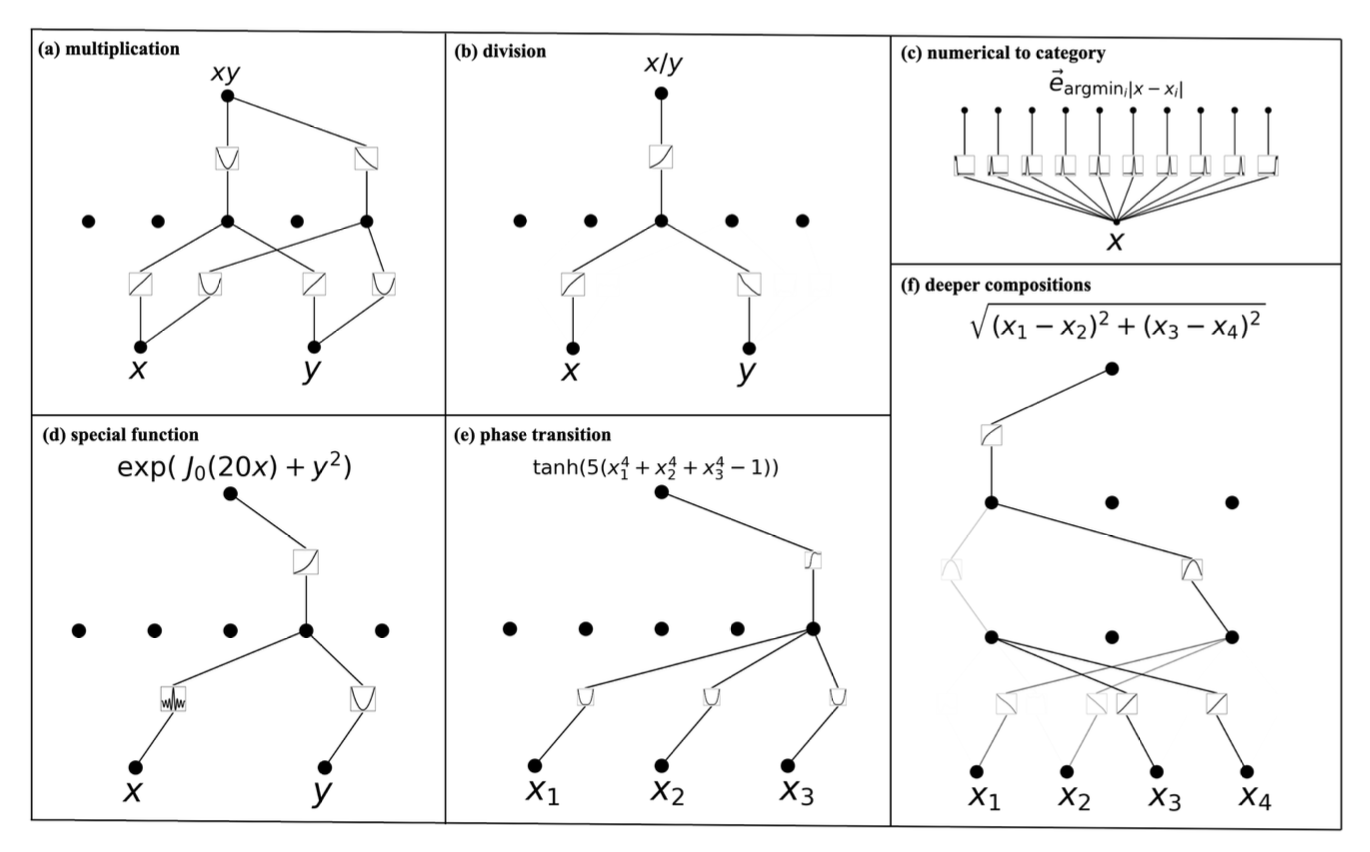
\includegraphics[width=10cm]{splines}}{\textit{Visualization of KANs trained on some input functions.}}
\end{frame}
\begin{frame}
    Note also that the shape of these KANs correspond quite well to the structure of the input function.
    \ffig{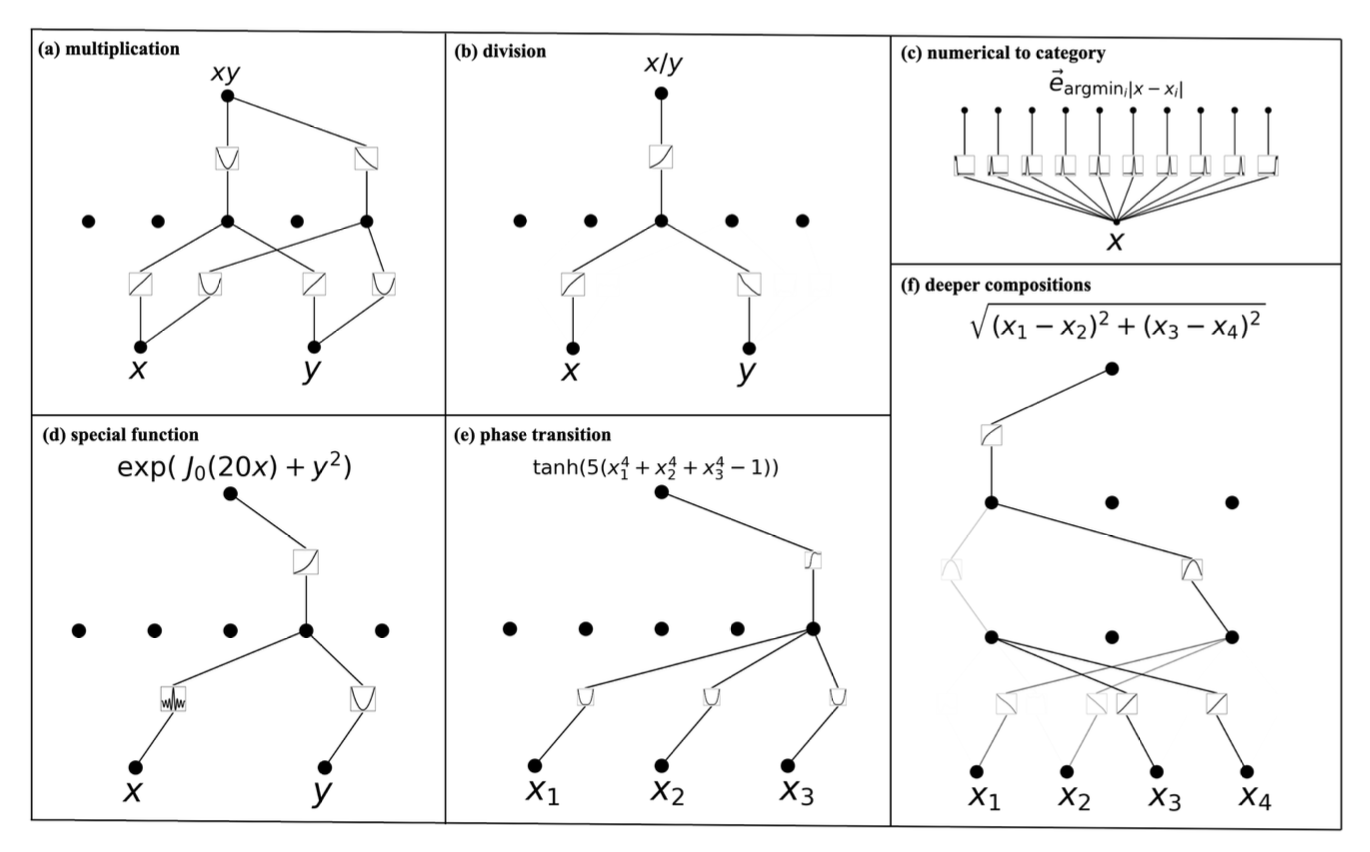
\includegraphics[width=10cm]{splines}}{\textit{Visualization of KANs trained on some input functions.}}
\end{frame}
\begin{frame}
    With a bit of regularization/sparsification in the objective function, 
    KANs can be trained to prune themselves down to a minimal depth and breadth, to the point that
    you can almost elicit an analytical function from the shape of the KAN. \\
    \ffig{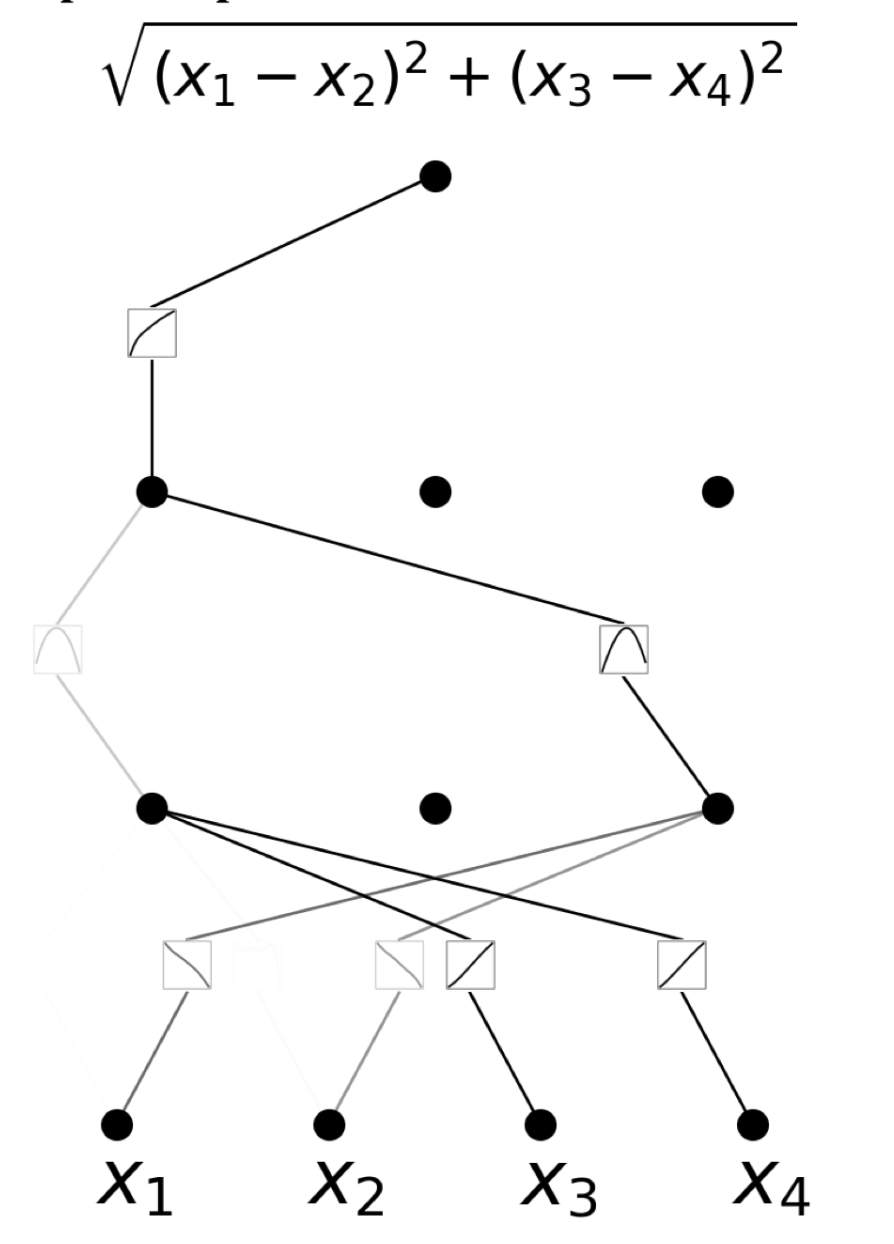
\includegraphics[width=2cm]{reg}}{\textit{Pruned KAN.}}
    There are a lot of really cool knot theoretic and physics-based examples in 
    the original paper, which I encourage you to peruse.
\end{frame}

\section{Why are we only hearing about KANs now?}
\begin{frame}
    There has been previous work on the application of Kolmogorov-Arnold to neural networks,
    but much of it predates modern concepts (like backpropagation and other efficient
    gradient methods). KAN training is also far more involved than MLP training. 
    \ffig{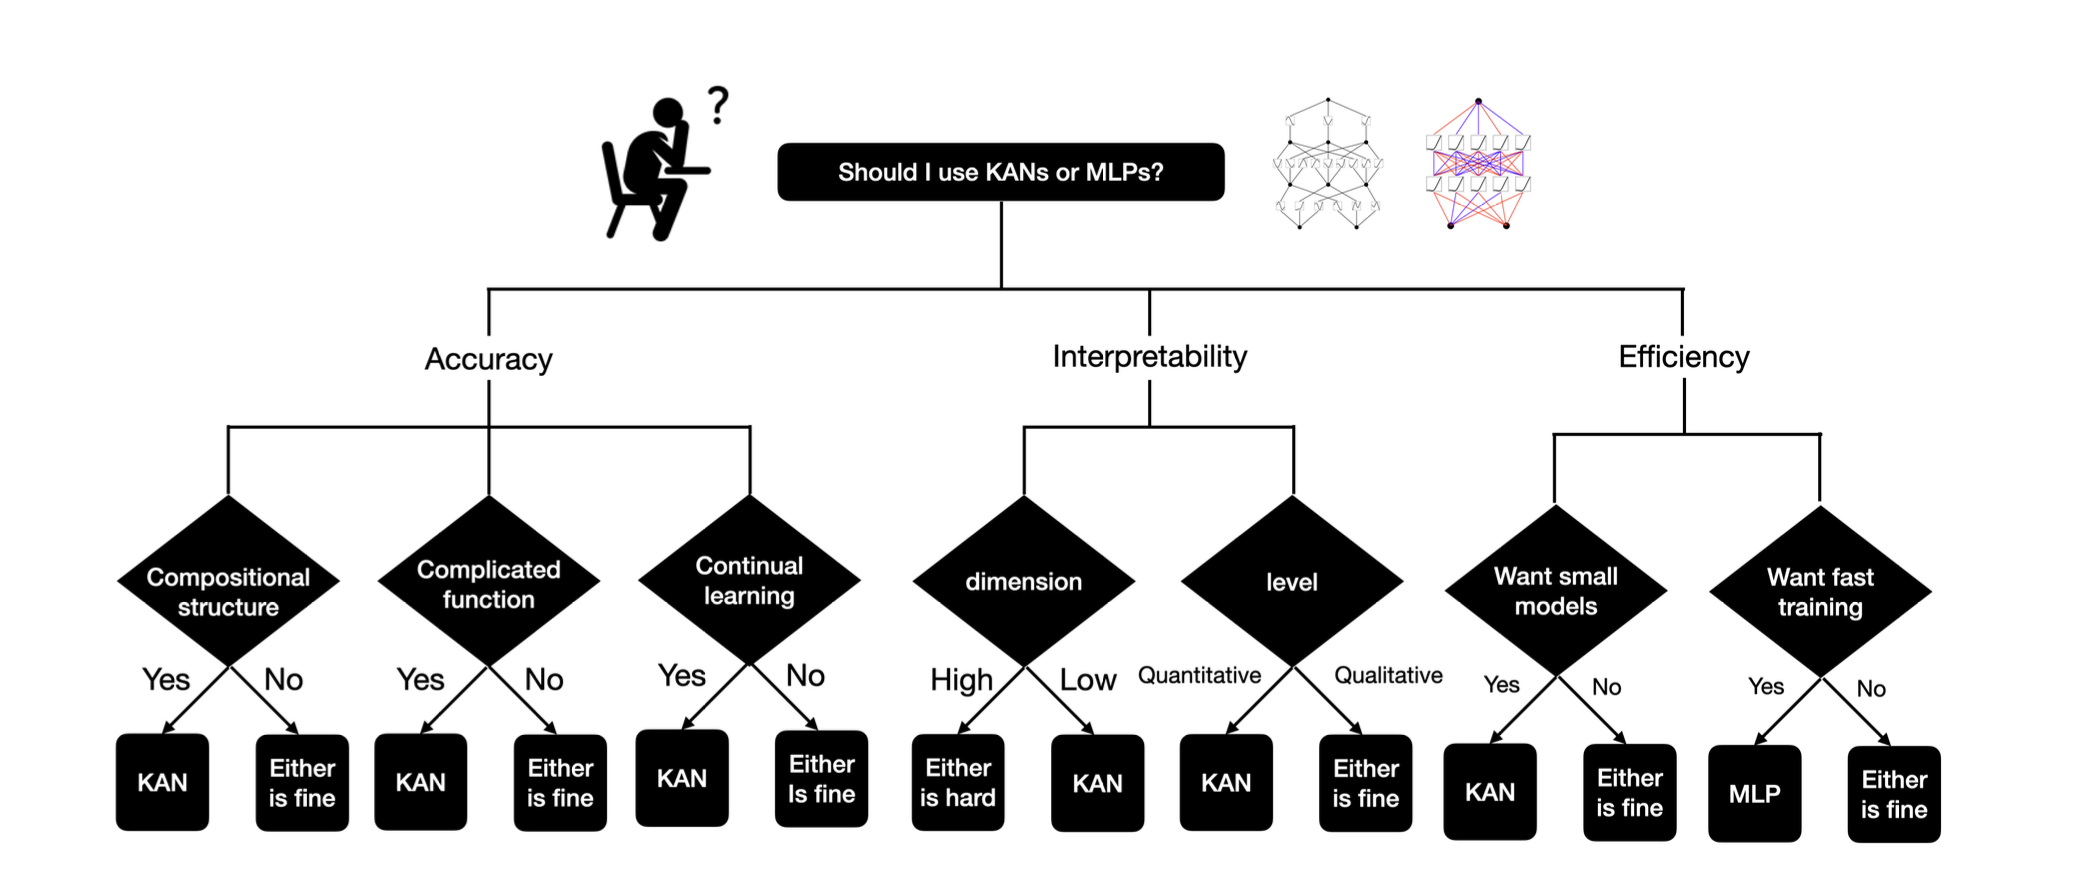
\includegraphics[width=10cm]{flow}}{\textit{Fun figure from Liu et al.}}
\end{frame}
\end{document}
